\documentclass[aps,prd,twocolumn,superscriptaddress,amsfont,amssymb,amsmath,nofootinbib,showpacs,balancelastpage]{revtex4-1}
%\documentclass[prd,superscriptaddress,twocolumn,floatfix]{revtex4}

\usepackage{graphicx,longtable,natbib,mathrsfs,color}
\usepackage{txfonts}

\newcommand{\bs}{\boldsymbol}
\newcommand{\diff}{{\mathrm d}}
\newcommand{\Cov}{\mathsf{C}}
\newcommand{\Fish}{\mathsf{F}}
\newcommand{\Cl}{\mathcal {C}}
\newcommand{\R}{\mathcal{R}}
\newcommand{\T}{\mathcal{T}}
\newcommand{\Msun}{M_\odot}
\newcommand{\lb}{\left\langle}
\newcommand{\rb}{\right\rangle}
\newcommand{\tcb}{\textcolor{blue}}
\newcommand{\tcr}{\textcolor{red}}

%
\def\apjl{Astrophys. J. Lett.}
\def\apjs{Astrophys. J. Suppl. Ser.}
\def\aj{Astron. J.}
\def\mnras{Mon. Not. R. Astron. Soc.}
\def\aap{Astron. Astrophys.}
\def\jcap{J. Cosmology Astropart. Phys.}
\def\aapr{Astron. Astrophys. Rev.}

\begin{document}

\addtolength{\hoffset}{-0.525cm}
\addtolength{\textwidth}{1.05cm}
\title{Reconstruction of Large Scale Structure by Nonlinear \tcr{Lagrangian} Displacement Fields}

\author{Hao-Ran~Yu}%\email{haoran@cita.utoronto.ca}
\affiliation{Kavli Institute for Astronomy and Astrophysics, Peking University, Beijing 100871, China}
\affiliation{Canadian Institute for Theoretical Astrophysics, University of Toronto, 60 St. George Street, Toronto, Ontario M5S 3H8, Canada}

\author{Ue-Li~Pen}%\email{pen@cita.utoronto.ca}
\affiliation{Canadian Institute for Theoretical Astrophysics, University of Toronto, 60 St. George Street, Toronto, Ontario M5S 3H8, Canada}
\affiliation{Dunlap Institute for Astronomy and Astrophysics, University of Toronto, 50 St. George Street, Toronto, Ontario M5S 3H4, Canada}
\affiliation{Canadian Institute for Advanced Research, CIFAR Program in Gravitation and Cosmology, Toronto, Ontario M5G 1Z8, Canada}
\affiliation{Perimeter Institute for Theoretical Physics, 31 Caroline Street North, Waterloo, Ontario, N2L 2Y5, Canada}

\date{\today}
%\date{Received \today; published -- 00, 0000}

\begin{abstract}
We investigate the ability of using nonlinear displacement field to reconstruct 
the primordial linear perturbations of the large scale structure. According to 
the linear Lagrangian perturbation theory, the first order primordial linear 
density field is given by the negative divergence of the displacement field. By 
running $N$-body simulations, we show that this \tcr{new} reconstruction algorithm recovers 
great amount of nonlinear information in the early universe. In reality, the 
displacement fields can be solved from only the final stage of the density 
fields. This demonstrates the potential to reconstruct baryonic acoustic oscillation (BAO) 
from current and future large scale structure surveys.

\end{abstract}

%\pacs{98.80.Es 95.36.+x}

\maketitle

\section{Introduction}\label{sec.intro}
Our universe starts from primordial Gaussian perturbations at a very early stage, 
and from those fluctuations, the gravitational instability drives the formation of 
the large scale structure (LSS) distribution of matter
\citep{1970A&A.....5...84Z,1985ApJ...292..371D}.
These structures grow 
linearly until the perturbations are large enough so that the first order 
perturbation theories are unable to analytically describe the LSS distributions 
\citep{2016JCAP...01..043M}. 
As a result, the final nonlinear LSS distribution contains higher order 
statistics, and thus makes it more challenging to be interpreted into basic
cosmological parameters. One such example is that, the baryonic acoustic oscillation (BAO)
scale can be used as a ``standard ruler'' to constrain the cosmic expansion history
and thus probes the dark energy properties \citep{2005NewAR..49..360E}, but
nonlinear evolution smears the BAO features and lowers the measurement
accuracy \citep{2005ApJ...633..560E,2012MNRAS.419.2949N}.
There are various attempts to recover earlier stages
of LSS, in which statistics are closer to Gaussian 
\citep{1992MNRAS.254..315W,2013MNRAS.436..759H}.
Because Gaussian fields can be adequately described by two-point statistics,
ideally after some recovery algorithms, more information can be extracted,
more straightforwardly, by power spectra or two-point correlation functions
\citep{2005MNRAS.360L..82R,2012MNRAS.421..832Y}.

Standard BAO reconstruction algorithms smooth the 
nonlinear density field on linear scale ($\sim$10 Mpc$/h$) and reverse the large 
scale bulk flows by a negative Zel'dovich linear displacement
\citep{2007ApJ...664..675E,2009PhRvD..80l3501N,2009PhRvD..79f3523P}. Here we propose a 
\tcr{new reconstruction method} that uses the nonlinear displacement field to recover the 
primordial density field. In the linear Lagrangian perturbation theory, the 
negative divergence of the the displacement field
$\bs\Psi(\bs q)$ respect to Lagrangian coordinates $\bs q$
gives the linear density field \tcr{\citep{2010PhDT.........4J}}.
Of course, the full displacement field $\bs\Psi(\bs q)$
is non-observable, as it requires the initial distributions of matter, however there are 
many techniques to estimate the nonlinear displacement field from a final 
distribution of matter. For example, when a homogeneous initial matter distribution 
is assumed, there is a unique solution of curl-less displacement field to relate 
the initial and final distributions without shell-crossing. This solution can be 
solved by a metric transformation equation \citep{1995ApJS..100..269P,1998ApJS..115...19P}.
\tcr{[Peacock, Goldberg?]}
In 1-dimensional (1D) case, the exact solution of \cite{1995ApJS..100..269P}
simplifies to an ordering of matter elements by Eulerian coordinates.
Zhu {\it et al.} \cite{2016arXiv160907041Z} apply this algorithm to the result
of an 1D simulation \citep{2016JCAP...01..043M} and obtain an estimated
displacement field $s(q)$, and find that \tcr{this new method} well recovers the linear
information and reconstructs BAO peak in correlation function. 
In 3D case, there are various techniques to obtain $\bs s(\bs q)$.
However one needs to carefully consider effects of curl, shell-crossing in 3D case.

Before these steps, we need to quantify the amount of linear information
that can be recovered from the full nonlinear displacement field $\bs\Psi(\bs q)$,
and further estimations $\bs s(\bs q)$ can be compared with this result.
In this paper we run a LSS $N$-body simulation and track the motion of
particles to obtain $\bs\Psi(\bs q)$. According to this we reconstruct the linear density
field and compare to the primordial density field of the initial
conditions. We describe the simulation and reconstruction algorithm in section
\ref{sec.method}, and we show the results in section \ref{sec.results}.
Discussion and conclusion are in section \ref{sec.discussion}.


\begin{figure}[b] \centering
  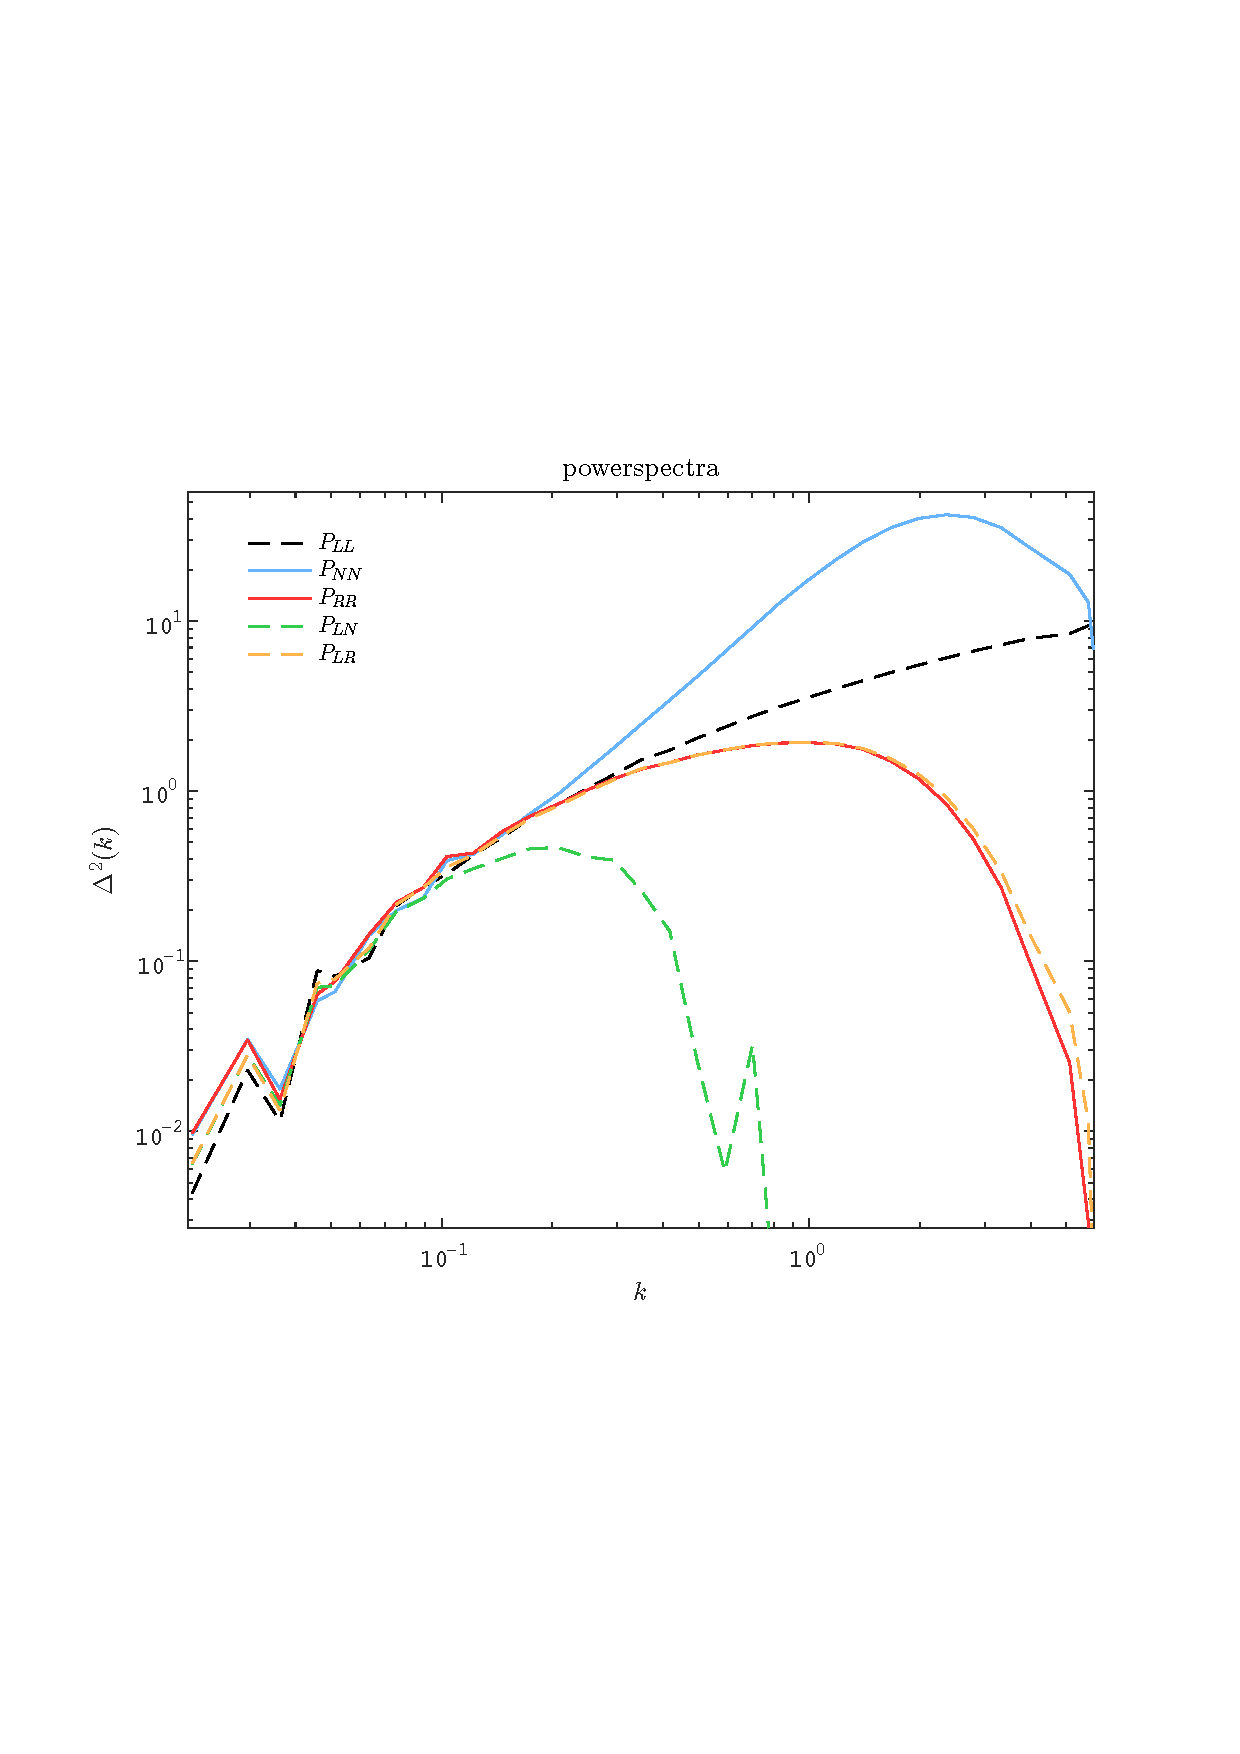
\includegraphics[width=1.0\linewidth]{fig1.pdf}
  \caption{Dimensionless auto- and cross- power spectra between nonlinear density field $\delta$, linear density field $\delta_L$ and reconstructed density field $\delta_R$.}
  \label{fig.1}
\end{figure}
\begin{figure}[t] \centering
  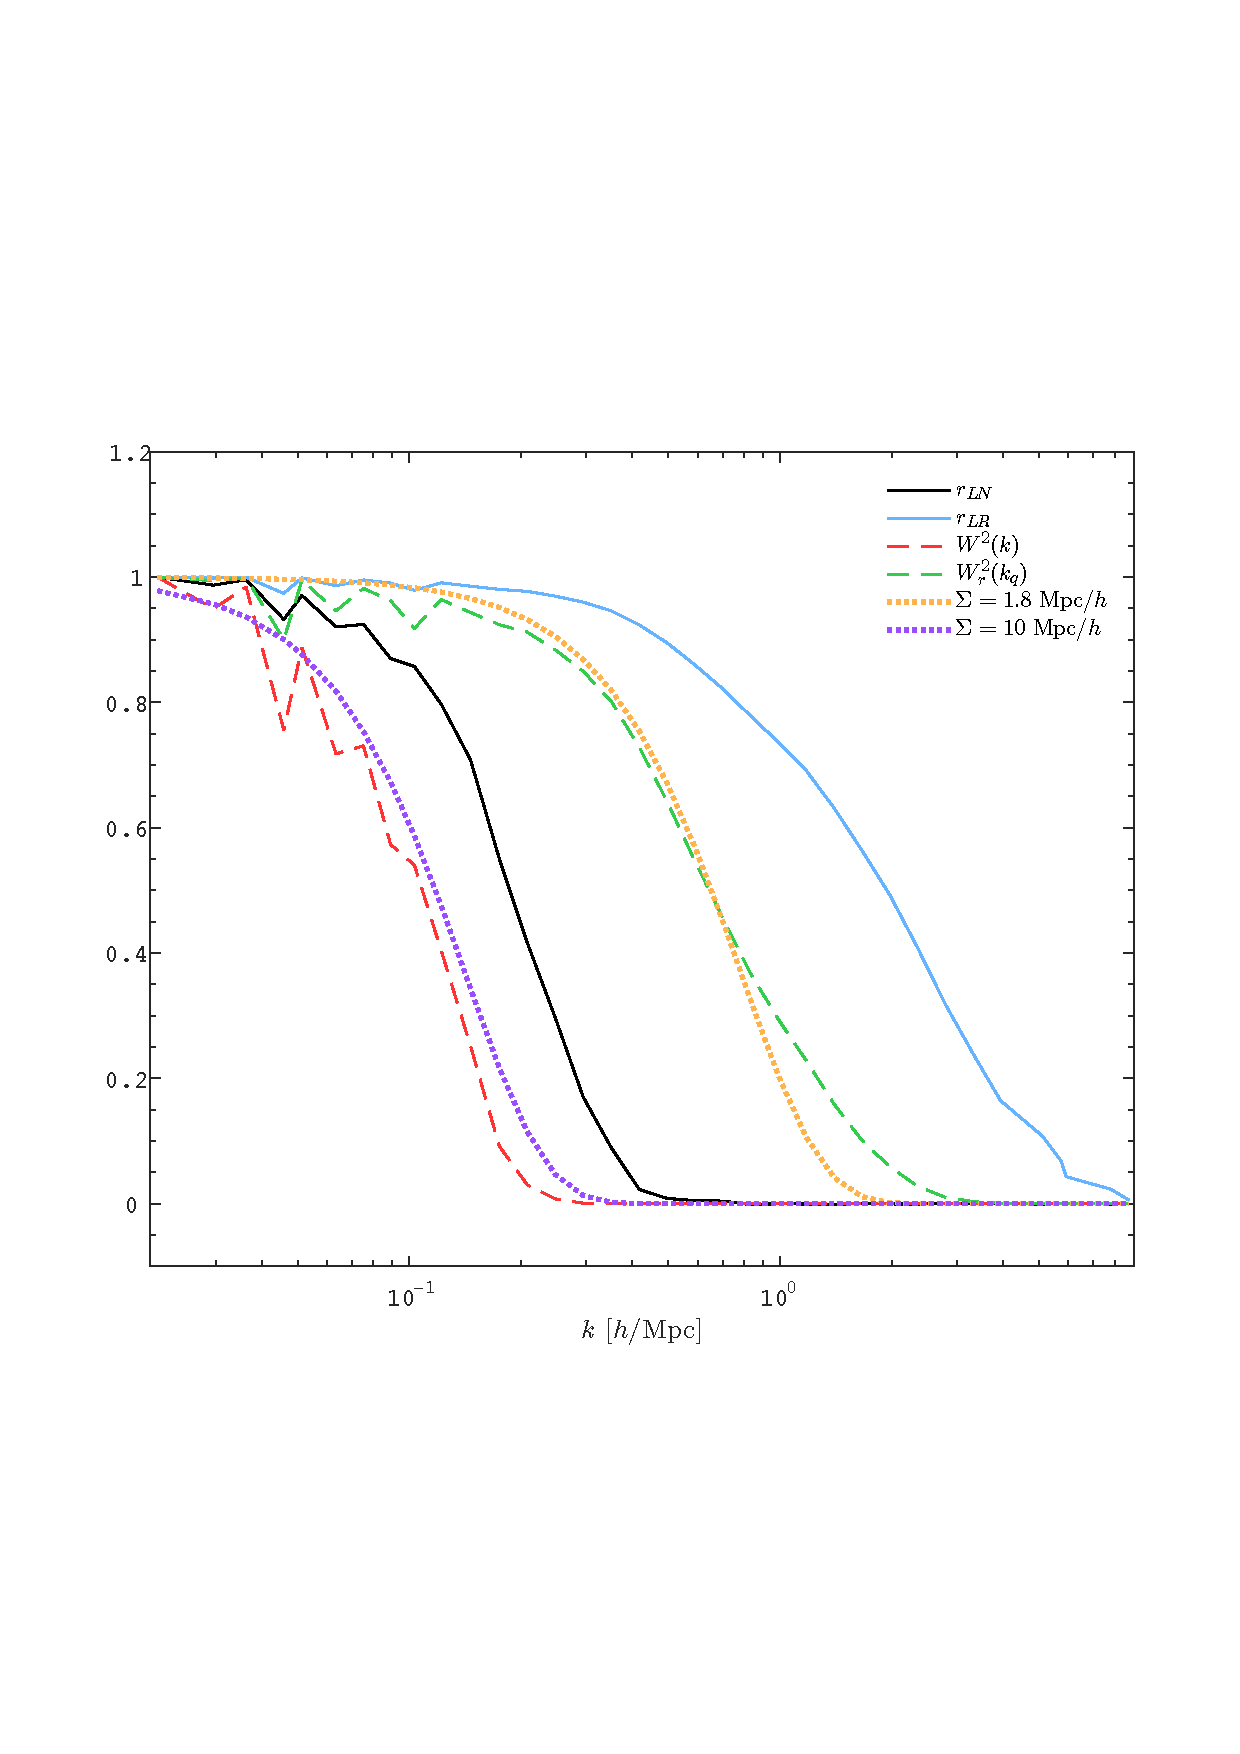
\includegraphics[width=1.0\linewidth]{fig2.pdf}
  \caption{Correlation functions $r(\delta_L,\delta)$ and $r(\delta_L,\delta_R)$
  (solid lines). Their
  damping of the power spectra $W^2$ (dashed lines),
  and their best fit BAO damping models (dotted lines).}
  \label{fig.2}
\end{figure}



\section{Method}\label{sec.method}
We show the LSS simulation and displacement field setups in section \ref{ss.sim},
and the reconstruction processes are presented in section \ref{ss.reco}.

\subsection{Simulation}\label{ss.sim}
We use the open source cosmological simulation code {\tt CUBE}%\footnote{github link of cafcube}
\citep{cafcube}.
Cosmological parameters are set as
$\Omega_m=0.27$, $\Omega_\Lambda=0.73$, $h_0=0.68$, $n_s=0.96$ and $\sigma_8=0.83$.
Initial conditions are generated at redshift $z=50$ 
using Zel'dovich approximation, and using a CLASS transfer function.
$N_p=512^3$ $N$-body particles are evolved via 
their mutual gravitational interactions to $z=0$, in a periodic box with $L=300$ 
Mpc$/h$ per side. The code is set to use standard a particle-mesh (PM) algorithm 
\cite{1988csup.book.....H} on a two-level mesh grids
(details see \cite{2013MNRAS.436..540H}) and cloud-in-cell
(CIC) is used in particle interpolations in force 
calculation and obtaining the density field $\rho({\bs x})$ in Eulerian coordinates 
${\bs x}$ at late stages. We use density contrast $\delta\equiv\rho/\lb\rho\rb-1$ 
to describe the density fluctuations. The primordial linear density field $
\delta_L$ is given by the initial stage and scaled to $z=0$ by the linear growth 
factor.

Two-point statistics of the density fields are quantified by the cross power 
spectrum $P_{ij}(k)\equiv(2\pi)^{-3}\langle|\delta_i(k)||\delta_j(k)|\rangle$, 
where subscripts $i,j$ may refer to linear ($L$), nonlinear ($N$), or reconstructed ($R$) density 
fields. When $i=j$ it reduces to the auto power spectrum $P_{ii}(k)$ or $P(k)$. We 
usually plot the dimensionless power spectrum $\Delta^2(k)\equiv k^3P(k)/2\pi^2$. 
The blue solid and black dashed curves in Fig.\ref{fig.1} show the power spectra of 
$\delta$ and $\delta_L$. Their difference shows the nonlinear evolution of LSS on 
small scales. Their cross power drops to a very low value, indicating a loss of 
linear information in the nonlinear power spectrum.

\subsection{Reconstruction}\label{ss.reco}
In the simulation, we use particle-ID (PID) to record the initial (Lagrangian) location ${\bs 
q}$ of particles, and the information is tracked until the $z=0$ and we can get the 
Lagrangian displacement vector ${\bs \Psi}\equiv{\bs x}-{\bs q}$ for every 
particle. Then these vectors are interpolated onto the initial Lagrangian 
coordinates ${\bs q}$ of particles and we get the displacement field ${\bs \Psi}
({\bs q})$.
The raw reconstructed density field is given by the differential motion of matter 
elements,
\begin{equation}
    \delta_R=-\nabla\cdot{\bs \Psi}({\bs q}).
\end{equation}
Because the reconstruction processes are implemented on Lagrangian coordinates,
$\delta_R$ takes the coordinates of $\bs q$ instead of $\bs x$.
We just write $\bs q$'s Fourier wave number
$k_q$ as $k$ to simplify the expression.
In Fig.\ref{fig.1} we show the power spectrum of $\delta_R$ and its cross power
with $\delta_L$. Despite of a lowered power of $\delta_R$ compared to $\delta$,
it has a much higher cross power with $\delta_L$ compared to $\delta_N$,
up to a relatively smaller scale (higher $k$).
\begin{figure}[t] \centering
  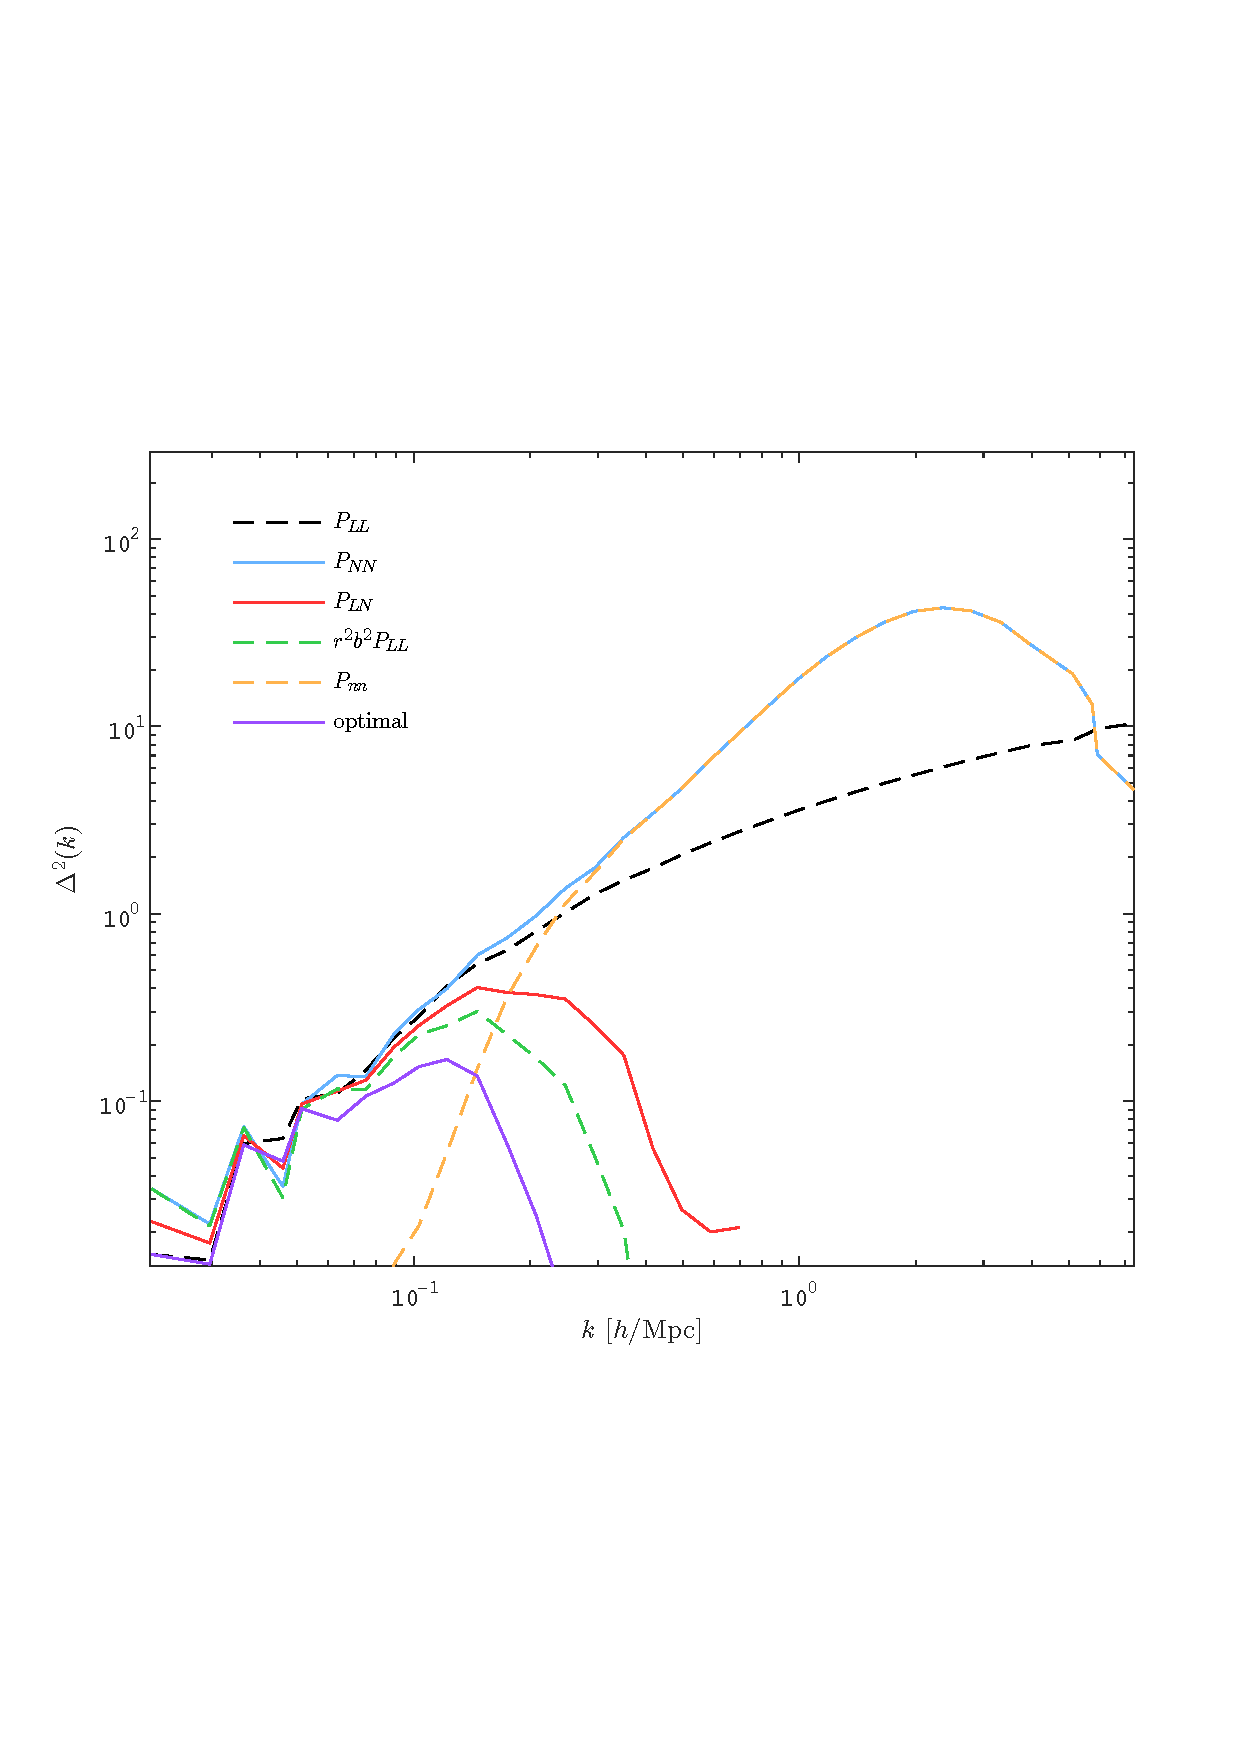
\includegraphics[width=1.0\linewidth]{fig3.pdf}
  \caption{Power spectra of the nonlinear density field and its
  filtered density field.}
  \label{fig.3}
\end{figure}

\begin{figure}[t] \centering
  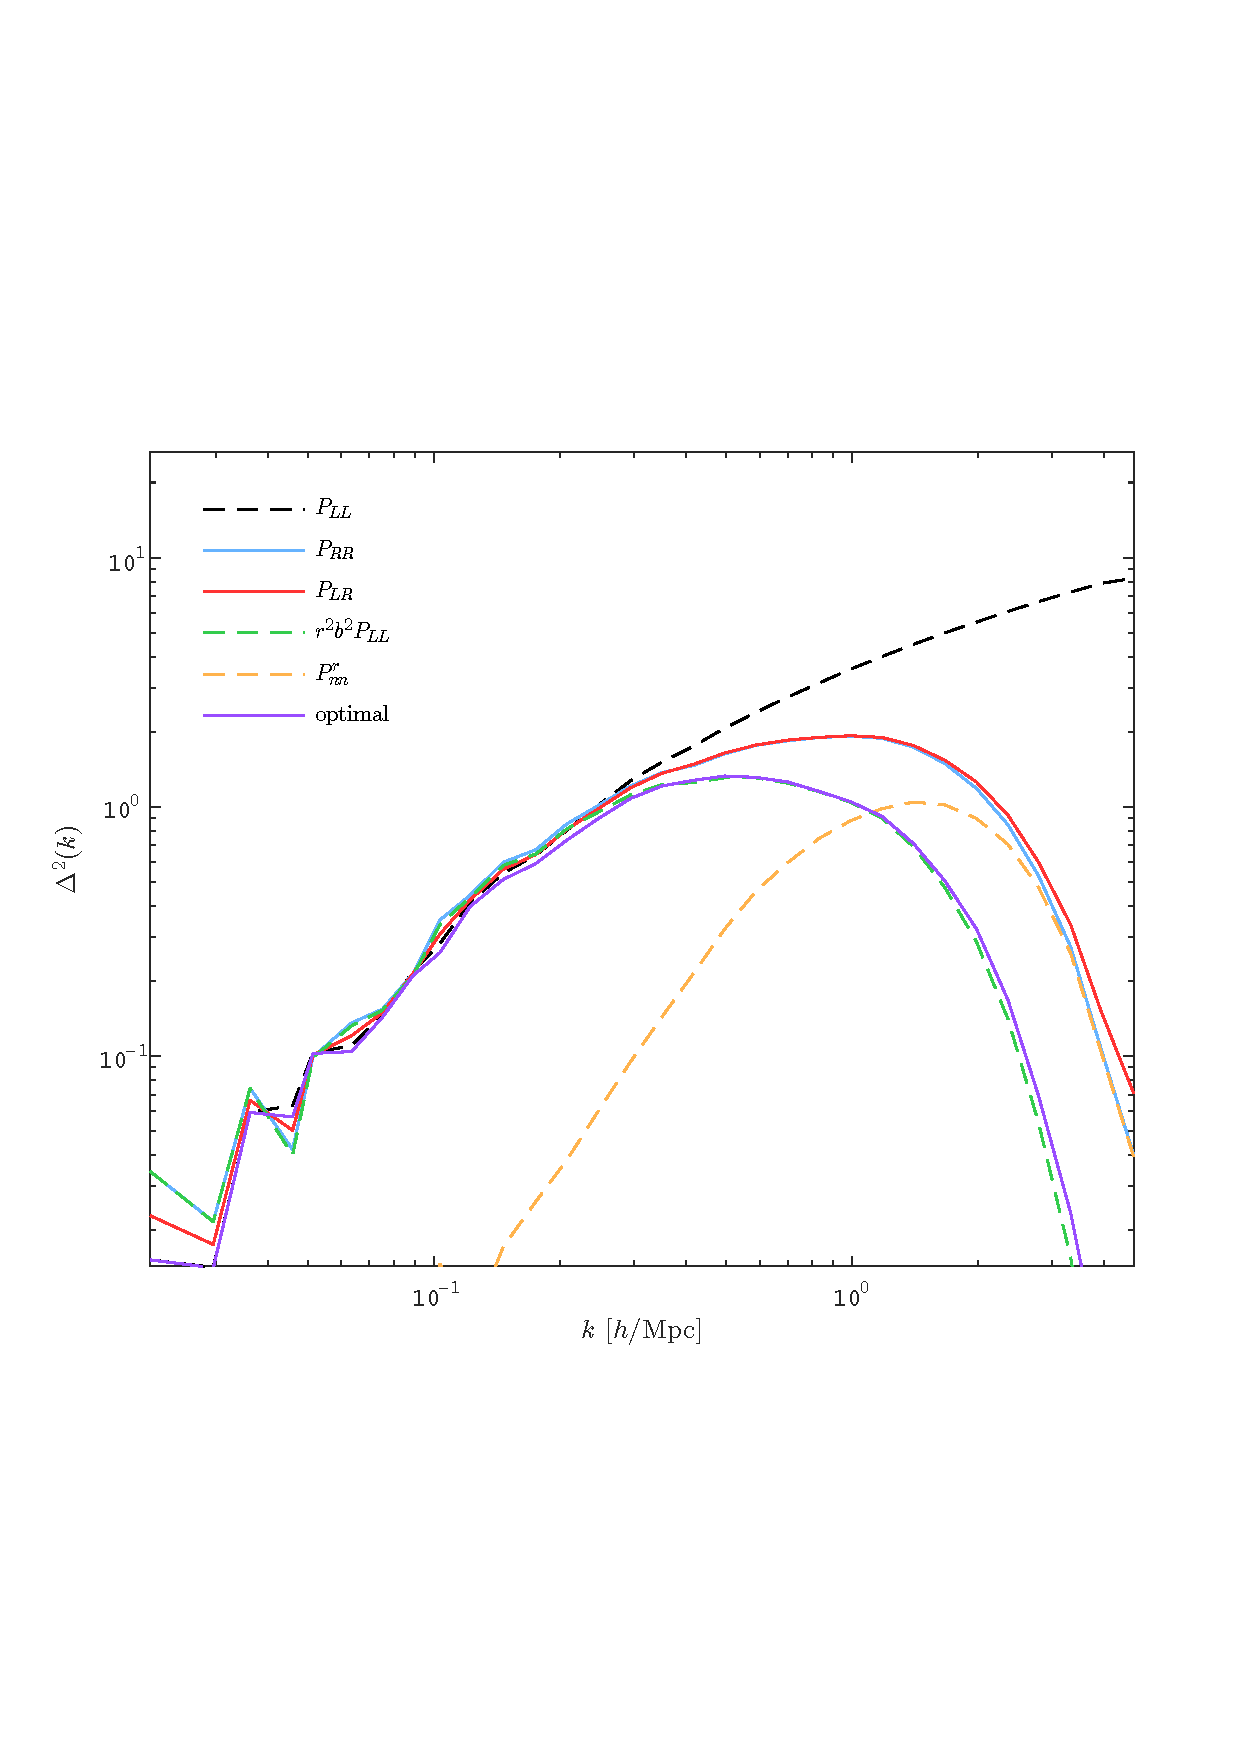
\includegraphics[width=1.0\linewidth]{fig4.pdf}
  \caption{Power spectra of the reconstructed density field and its
  filtered density field.}
  \label{fig.4}
\end{figure}

To quantify the linear information in the reconstructed density field, we decompose $\delta_R$ in Fourier space as
\begin{equation}\label{eq.decompose}
    \delta_R(k)=r'\delta_L+\delta_N,
\end{equation}
where $r'\delta_R$ is completely correlated with linear density $\delta_L$. Correlating equation (\ref{eq.decompose}) with $\delta_L$ gives
\begin{equation}
    P_{LR}=r'P_{LL}+P_{LN},
\end{equation}
where $P_{ij}\equiv\langle\delta_i\delta_j\rangle$ denotes the cross power 
spectrum. Since $\delta_N$ is uncorrelated with $\delta_L$, $P_{LN}=0$. With the 
definition of cross correlation coefficient $r(\delta_L,\delta_R)\equiv P_{LR}/\sqrt{P_{LL}P_{RR}}$ 
and bias $b^2=P_{RR}/P_{LL}$, we solve $r'=P_{LR}/P_{LL}=rb$. We plot the cross 
correlation coefficient $r_{LN}$ and $r_{LR}$ in Fig.\ref{fig.2}. Clearly, $
\delta_R$ contains much more linear information on smaller scales.

According to equation (\ref{eq.decompose}), the auto power spectrum is decomposed as
\begin{equation}\label{eq.power}
    P_{RR}=r^2b^2P_{LL}+P_{NN},
\end{equation}
and $P_{NN}=(1-r^2)P_{RR}$. Then we construct a Wiener filter to filter out the uncorrelated part in $\delta_R$:
\begin{equation}
    W(k)=\frac{r^2b^2P_{LL}}{r^2b^2P_{LL}+P_{NN}}=r^2.
\end{equation}
The Wiener filters are also plot in Fig.\ref{fig.2}. The estimated linear density, or the optimal reconstructed density is given by
\begin{equation}
    \tilde\delta_R=Wb^{-1}\delta_R.
\end{equation}
The full filters $Wb^{-1}$ are also plotted in Fig.\ref{fig.2}.
The optimal reconstructed power spectrum is given by
\begin{equation}\label{eq.opt}
    \tilde P=W^2b^{-2}P_{RR}=W^2P_{LL}+W^2b^{-2}P_{NN}.
\end{equation}
The $W^2$ describes the damping of the linear power spectrum.

\section{Results}\label{sec.results}
Fig.\ref{fig.2} shows the cross correlation functions,
damping factors $W^2(k)$ for the optimal filtered 
nonlinear and reconstructed density fields.
We can see that the cross correlation $r_{LR}$ is recovered to
nearly an order of magnitude smaller scales compared to $r_{LN}$.
We also fit the Gaussian BAO damping model $
{\mathcal D}(k)=\exp(-k^2\Sigma^2/2)$ and give $\Sigma=1.8$ Mpc$/h$ and $\Sigma=10$ 
Mpc$/h$ for nonlinear and reconstructed fields.
We repeat the analysis with various box sizes,
and the results are consistent.

In Fig.\ref{fig.3} and Fig.\ref{fig.4} we show the power spectrum
decomposition by equation (\ref{eq.power}) for both $\delta_N$ 
(with subscripts ``$_R$'' replaced by ``$_N$'') and $\delta_R$.
In Fig.\ref{fig.3} we can see that, on scales $k>0.2\ h/$Mpc,
$P_{NN}$ term dominates the power spectrum due to a low correlation
between $\delta_L$ and $delta_N$. The optimal filtered power spectrum
damps quickly on small scales. In comparison, in Fig.\ref{fig.4},
$P_{NN}$ starts to dominate on scales $k>1\ h/$Mpc. As a result, the
optimal filtered reconstructed power spectrum
(by equation (\ref{eq.opt})) is much higher.

\section{Discussion and conclusion}\label{sec.discussion}
We extract the actual displacement field of matter elements in cosmological $N$-body
simulations, and use this displacement field in Lagrangian coordinates to reconstruct
the primordial linear perturbations. The result shows a prominent improvement from
$r_{LN}$ to $r_{LR}$ in Fig.\ref{fig.2} -- recovering the lost linear information on
nearly an order of magnitude smaller scales.
This is achieved by implementing differential movement information
of matter elements on Lagrangian coordinates, rather than on
Eulerian coordinates. This result illustrates the feasibility
of using estimated displacement field $\bs s(\bs q)$ to reconstruct primordial linear
density field. A straightforward example of a estimation of $\bs s(\bs q)$
is given by \cite{1995ApJS..100..269P,1998ApJS..115...19P}.
More complicated algorithms can be found in \tcr{[cite]}, where
shell-crossing effects are also considered. In reality, one needs
to consider all aspects including vorticity, shell-crossing, bias, noise
and data complexities. The impact of these factors can be quantitatively
compared with the impact of different estimation methods, and with
the exact solution by $N$-body simulations.

\tcr{Is this reconstruction method optimal? Is there any other better methods?}

\tcr{A proper name of this method?}

\section*{Acknowledgements}
HRY acknowledges General Financial Grant from the China Postdoctoal Science Foundation No.2015M570884.

%\bibliographystyle{apsrev4-1}
\bibliographystyle{h-physrev3}
\bibliography{../haoran_ref}

\end{document}
